\documentclass[a4paper,12pt]{article}
\usepackage[top=1.2in, bottom=1in, left=1.4in, right=1.4in]{geometry}
\usepackage{graphicx} 
\usepackage{hyperref}
\usepackage{algorithm}
\usepackage{algpseudocode}
\usepackage{amsmath,amssymb}
\usepackage{colortbl}
\graphicspath{ {pics/} }
\usepackage{array}
\title{Lost and Found\\ {\normalsize A Software Engineering Lab Project\\} \vspace{6cm}Software Design Document (SDD)\\\textit{Ver 1.0}\vspace{6cm}}
\author{Team 3\\\\Ahamed P A (B130121CS)\\Simsarul Haq Vengasseri (B130461CS)\\Durge Snehal Pradeep (B130839CS)\\Rohit Garlapati (B110316CS)\\Upasana Bai Asokan (B130488CS)\\\\ \textbf{Mentor: Ms. Anu Mary Chacko}}
\renewcommand{\listfigurename}{Index of Figures}
\newcommand{\specialcell}[2][c]{%
  \begin{tabular}[#1]{@{}c@{}}#2\end{tabular}}
\begin{document}
\begin{titlepage}
\maketitle
\thispagestyle{empty}
\end{titlepage}
\pagebreak
\thispagestyle{empty}
\begin{center}
{\large \textbf{Revision History\vspace{1cm}}}
\begin{tabular}{|c|c|c|c|}
 \hline
 \rowcolor[gray]{0.8}
 \textbf{Version}&\textbf{Date}&\textbf{Author}&\textbf{Change Description}\\
 \hline
 0.1&28/02/2016&\specialcell{\\Akshay K Patil\\Arjun Krishnamoorthy\\Azharullah Shariff\\Harish Paul Thavisi\vspace{0.2cm}}&Initial release\\
 \hline
 1.0&09/03/2016&\specialcell{\\Ahamed P A\\Simsarul Haq Vengasseri\\Durge Snehal Pradeep\\Upasana Bai Asokan\\Rohit Garlapati\vspace{0.2cm}}&Revised release\\
 \hline
\end{tabular}
\end{center}
\pagebreak
\thispagestyle{empty}
\tableofcontents
\pagebreak
\thispagestyle{empty}
\listoffigures
\pagebreak
\section{Introduction}
\subsection{Purpose}
This document will outline the design of the 'Lost and Found' Application. It contains specific information about the actions taken by the user, the corresponding output by the application and other functions. It specifies the details about the interaction between various components to meet the desired requirements. It provides a detailed view of the system's design to understand the working of the system. 
\subsection{Scope}
This document is based on the SRS Release 1.0 of the 'Lost and Found' Application.  It contains details about how the design will implement the non-functional and functional requirements mentioned in the Software Requirements Specification (SRS) document. 
\subsection{Intended Audience}
This document is written to address the team that will perform the implementation task for this application and for the perusal of Dr. Vinod Pathari and the client, Kurian Jacob.
\subsection{Definitions, Acronyms and Abbreviations}
\begin{itemize}
\item DBMS - Database Management System.  A programmable interface which provides a common layer of abstraction between a physical database and a user or external program.
\item LFA - Lost and Found Application.
\item NITC - National Institute of Technology, Calicut.
\end{itemize}
\subsection{System Overview}
The project is a 'Lost and Found' item manager accessible to the students of NITC. It aims to replace the "Lost and Found" desk at NITC. It does so by providing a platform for users to post details of their missing items and browse through posts made by other users who have found some lost property. The app relies primarily on e-mail communication between the two parties through their nitc e-mail IDs and optionally Facebook and/or contact numbers. No third party involvement is present in the whole process of reclaiming the item. All the data is stored in the DBMS associated with the application.\\
The app allows the users to:\\
\begin{itemize}
\item Post details of lost items
\item Post details of found items
\item Resolve their posts
\item Subscribe to categories of lost articles
\item Browse through "Lost" and "Found" feeds
\item Manage their user profiles
\item Report inappropriate posts and users
\end{itemize}
\section{Design considerations}
This section describes many of the issues which need to be addressed or resolved before attempting to devise a complete design solution.
\subsection{Assumptions and Dependencies}
\begin{itemize}
\item The app requires a working internet connection
\item The app must be compatible with Android 4.0 and above.
\item Users are required to have an NITC Email ID in order to register.
\item The App must be able to integrate with the NITC mail system for communication and validation purposes.
\item It requires the optional integration of Facebook for contact details.
\item The app relies on Google Maps to specify the exact location where the item was found.
\item Users can trust this app to claim their missing property without the need of an intermediary, in an ideal scenario. 
\item The security of the system is based on password-based authentication of the user's NIT-C e-mail ID. 
\end{itemize}
\subsection{General Constraints}
\begin{itemize}
\item An Android mobile device (4.0 or later), preferably with a GPS tracker is required. 
\item Users can create their accounts only after verifying their identity using their valid NITC Email ID. 
\item A user can create only one account for his NITC ID. 
\item The application is meant for reporting items lost or found within the NITC campus only.
\end{itemize}
\subsection{Development Methods}
The methodology majorly used in the design of this application was the Waterfall Model, in which the software design is organically put together from the Software Requirements Specification created in the previous stage of the software development process. The construction/testing/implementation soon follows according to the model, finally culminating in the maintenance stage.
\section{System Architecture}
This system will follow a three-tier architectural style, i.e. it will be organized into three layers: the interface layer, the application layer and the storage layer. The interface layer will be the graphical user interface that allows the users to interact with the system. It will be implemented using the Android Studio, a Java Media Framework. The application layer will contain the logic and rules for storing data of users and items in the database layer and also retrieving it in accordance with the user's needs and this layer provides logic or algorithms for matching the items and retrieving the recommendations. This is the layer that will contain the data file parsers and will allow controlled access to the data files. Finally, the storage layer will store the metadata required for the system.
\paragraph{}
The three-tier architecture style shall be used because it not only separates the user interface and the metadata, but also provides an application logic layer. The application layer provides a middle layer that allows the data files and the GUI components to be loosely coupled. The application layer has to be modified if there are any changes to the format of the data files and the interface layer will need little or no modification. This will make it easy for clients of this software to modify the data file format and attributes for further research purposes if they wish to do so. This layer makes the system more maintainable and reusable and also hides the complexity of processing data from the users.
\paragraph{}
The system architecture for 'Lost and Found' is concerned with how users of the application can view the lost or found items that are in the database and resolving in the case of match. To describe this system architecture the following architectural view.
\newpage
\begin{figure}[h!]
  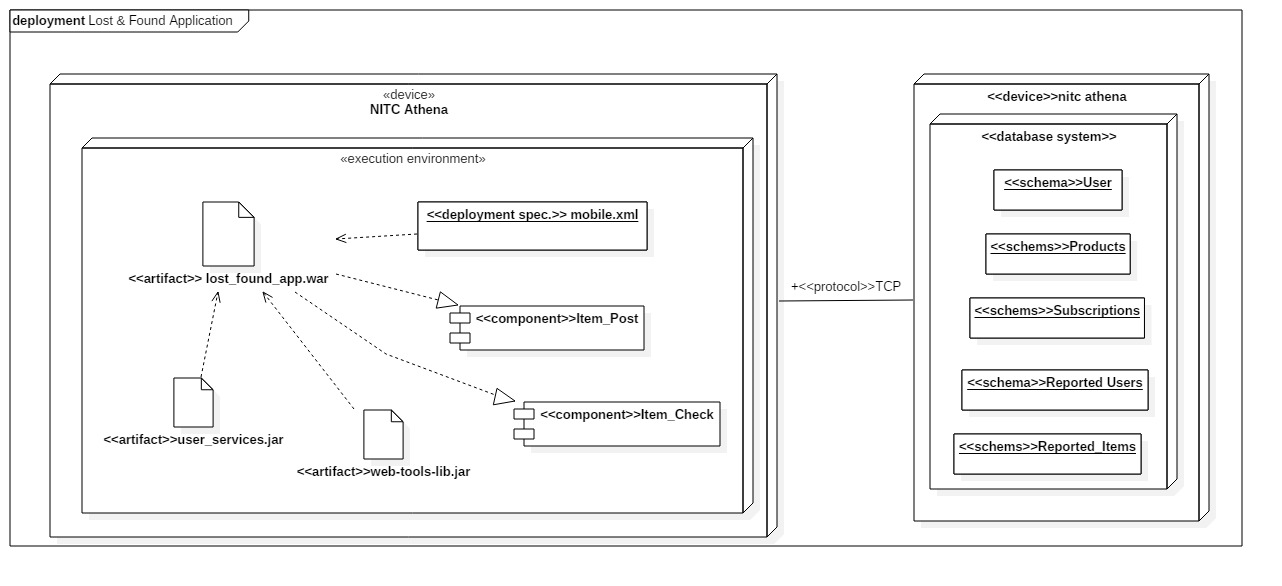
\includegraphics[width=1\textwidth]{deployment}
  \caption{Deployment Diagram}
\end{figure}
\begin{figure}[h!]
  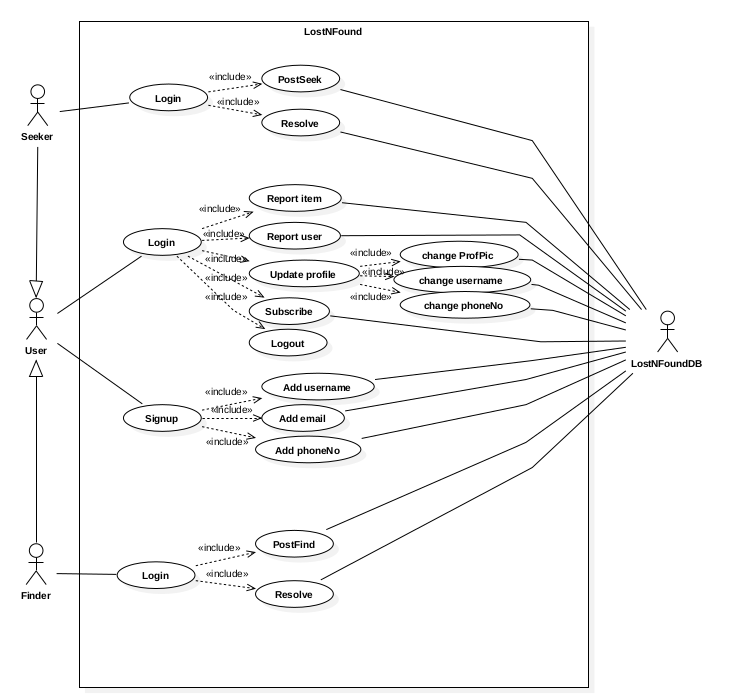
\includegraphics[width=1\textwidth]{use}
  \caption{UseCase Diagram}
\end{figure}
\section{Detailed System Design}
\subsection{View of Product Classes}
\begin{figure}[h!]
  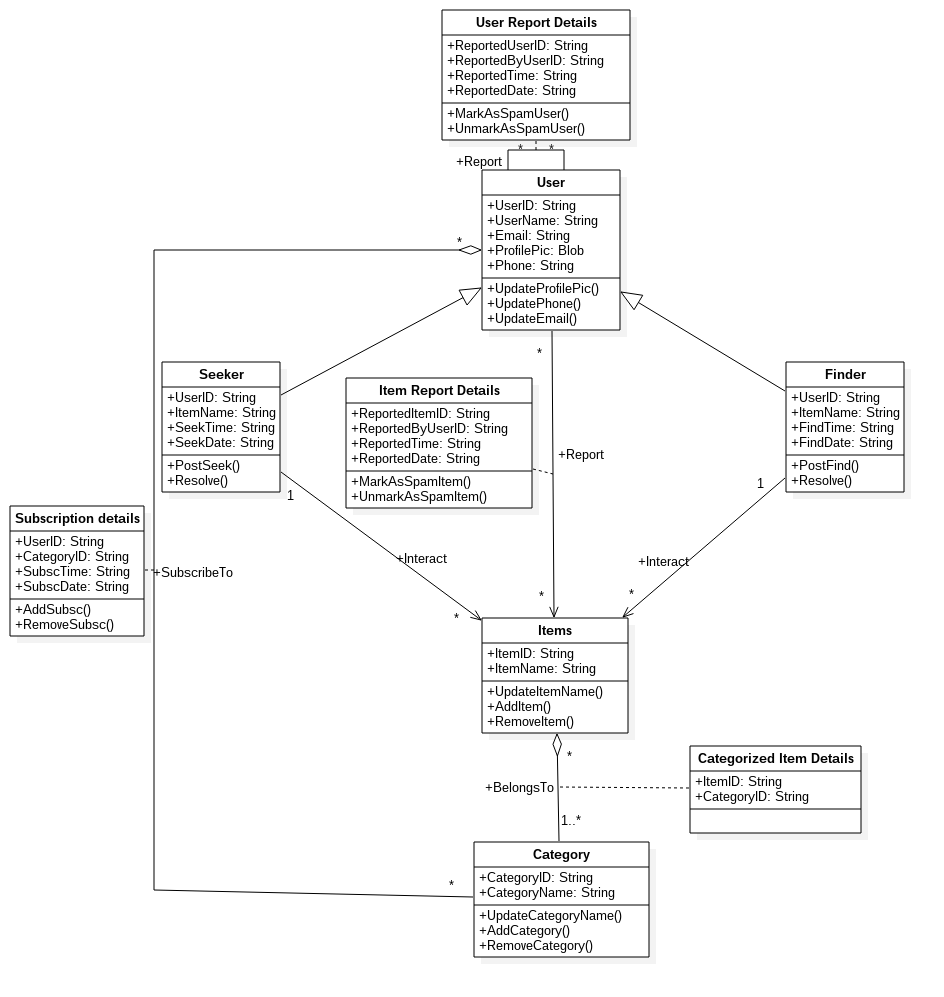
\includegraphics[width=1\textwidth]{class}
  \caption{Class Diagram}
\end{figure}
\subsection{Classification}
\begin{itemize}
\item Subsystem: The subsystems in our application are the Application Interface, the Database and the relevant Actions. 
\item Function: The functions in our application are 'Posting an item', 'Resolving a post', 'Reporting a user/item', 'Subscribing to or Unsubscribing from a category' and 'Authentication'. 
\item Class - The classes in our application are user and items. 
\item Module - The module in our application is the items feed.
\end{itemize}
\subsection{Definition}
\begin{itemize}
\item Post Details: A user can post details of the articles that they have found/lost. 
\item Resolving a post: Once the user has successfully reclaimed/returned his lost/found property, he can resolve the post. 
\item Reporting a user/item: If a user has found that a post/item is invalid/spam content, he can flag that specific post/user as inappropriate. 
\item Subscribing/Unsubscribing: A user can manage his subscriptions by subscribing/unsubscribing a category to receive/stop receiving notifications about items in that category.
\item Authentication: A user has to do a one-time authentication using his NITC Gmail ID on accessing the application for the first time. 
\item User: The class 'user' is a collection of information about all the users who have logged in to the application.
\item Items: The class 'items' is a collection of information about all the items that have been posted as lost or found in the application. 
\item Items feed: The items feed is a view (available to the users) of all the items that have been posted as lost or found in the application. 
\item Application interface: The subsystem 'application interface' is the GUI for the user to access the application.     
\item Database : The subsystem 'Database' is the collection of information of all the users and items in the application 
\item Actions: The subsystem 'Actions' is a set of all the functionalities a user of the application can have.
\end{itemize}
\subsection{Responsibilities}
\begin{itemize}
\item Post Details : This component will get the lost/found item details from the user and store it into the database 
\item Resolving a post: This component will remove the resolved item entry from the database. 
\item Reporting a user/item: This component will flag each spam item/user. 
\item Subscribing/unsubscribing a category: This component ensures that the user is notified about all the item updates in a particular category he has subscribed to. 
\item Authentication: This component will ensure that only people with valid NITC Email ID are able to access the application. 
\item Items feed: The items feed gets all the unresolved items from the database.
\end{itemize}
\subsection{Constraints}
For all the component interactions, authenticating with a valid NITC email id is a precondition. Constraints specific to these components are:\\
\begin{itemize}
\item Post Details: The system stores this information and the user is redirected to the 'Lost' Feed. There should be a character limit on the product description provided.  
\item Resolving a post: The system stores this information and the user's homepage is refreshed.
\item Reporting a user/item: A red dot appears next to the post/user profile which serves as a spam indicator. 
\item Subscribing/Unsubscribing a category: The system updates this information and refreshes the Homepage. 
\item User: The class 'user' is a collection of information about all the users who have logged in to the application. 
\item Items: The class 'items' is a collection of information about all the items that have been posted as lost or found in the application. 
\item Items feed: Users are able to view the feed.
\end{itemize}
There should be synchronization between the database and items feed (whenever there is an item resolve or an item report, the item feed should update immediately).
\subsection{Composition}
Most of the components in the application are functions and the others are atomic. Hence, they cannot be further decomposed. So, there are no sub-components.
\subsection{Uses/Interactions}
All the components will use the authentication component.
\begin{itemize}
\item Post Details: This component uses the 'application interface' to get the lost/found item and its details from the user. This component is used by the 'database' (both user and items).    
\item Resolving a post: This component uses the 'item feed' to resolve the post. It is used by the 'database' to remove the resolved item. 
\item Reporting a user/item: This component uses the 'items feed' to flag the user/item. It is used by the 'database' to flag that user/item.  
\item Subscribing/unsubscribing a category: This component uses the 'application interface' (manage subscriptions button) for the user to subscribe/unsubscribe a category. It is used by the 'database' to keep track of a user's subscriptions. 
\item User: This component is used by the 'report user' component. 
\item Items: This component uses the 'post details' component to update the items collection. This component is used by the 'report user' and 'resolve post' components.  
\item Items feed: This component uses the 'database' to display all the unresolved items in the application. This component is used by 'resolve item' and 'report item components'. 
\item Application interface : This component is used by 'post details', 'subscribing/unsubscribing a category', 'reporting a user/item', 'authentication' and 'resolving' components.    
\item Database: This component is used by all the functions to make the necessary updates. 
\item Actions: This component uses the 'database'.
\end{itemize}
\begin{figure}[h!]
  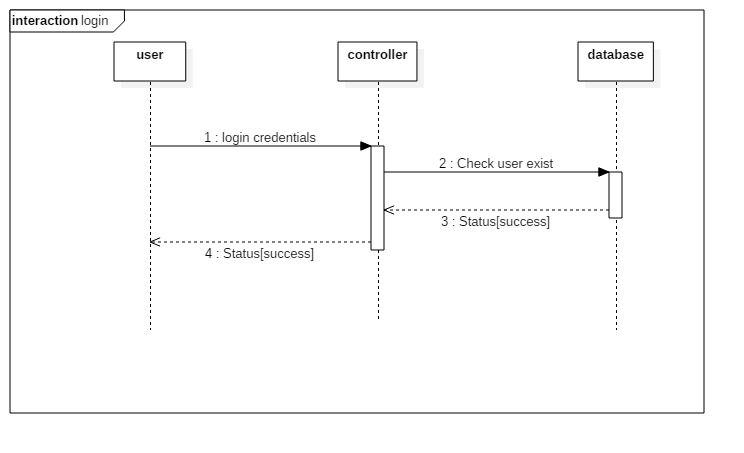
\includegraphics[width=1\textwidth]{login}
  \caption{Sequence Diagram for Login}
\end{figure}
\begin{figure}[h!]
  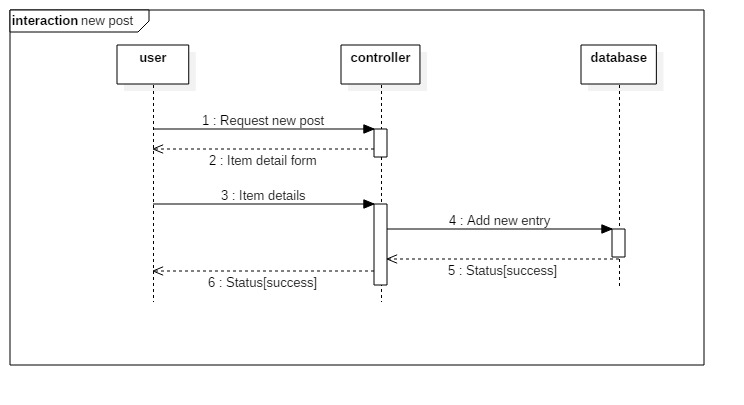
\includegraphics[width=1\textwidth]{newpost}
  \caption{Sequence Diagram for a New Post}
\end{figure}
\begin{figure}[h!]
  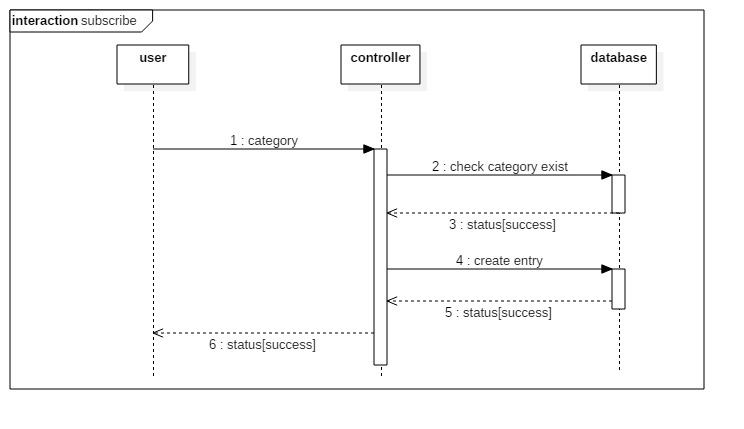
\includegraphics[width=1\textwidth]{subscribe}
  \caption{Sequence Diagram for Subscribe}
\end{figure}
\begin{figure}[h!]
  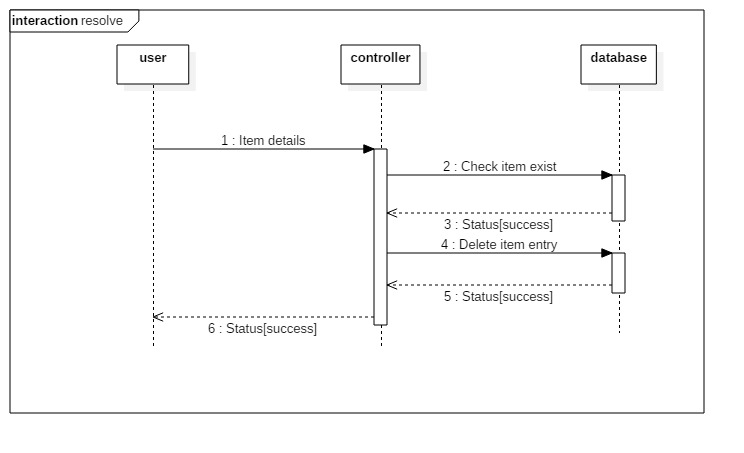
\includegraphics[width=1\textwidth]{resolve}
  \caption{Sequence Diagram for Resolve}
\end{figure}
\begin{figure}[h!]
  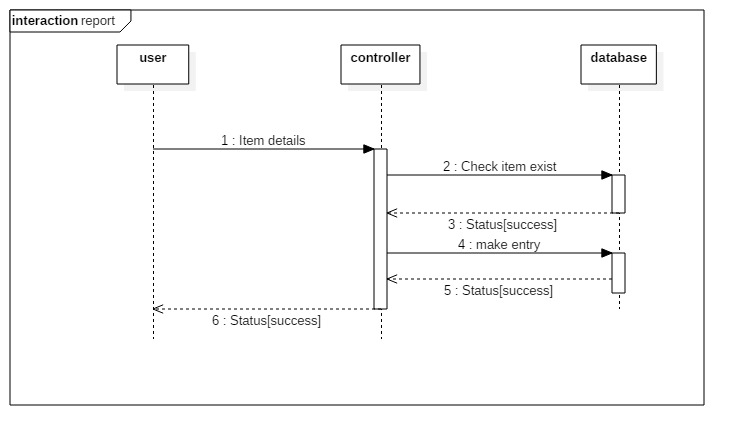
\includegraphics[width=1\textwidth]{report}
  \caption{Sequence Diagram for Report}
\end{figure}
\subsection{Resources}
All the functions manage the database and all the components need the database. There are no deadlock/race conditions that can occur at any point.
\subsection{Processing}
\begin{itemize}
\item Post Details: When a user clicks the 'post details' button, the 'post details' component gets the 'item details' and stores it in the 'database'.
\item Resolving a post: This component deletes the 'resolved item' from the 'database'. 
\item Reporting a user/item: This component flags the 'reported user/item' and toggles a flag counter corresponding to that particular item/user in the 'database'. 
\item Subscribing/unsubscribing a category: This component manages the user's notifications about the item updates in the subscribed categories. 
\item Authentication: A user has to do a one-time authentication using his NITC Gmail ID on accessing the application for the first time. 
\item Items feed: It uses the 'database' to display all the unresolved items. 
\item Application interface: It provides a GUI for all the application functionalities so that necessary actions can be performed and information can be sent to the 'database'. 
\item Database: Information received from the application interface is updated/added.
\end{itemize}
{
\begin{figure}[h!]
  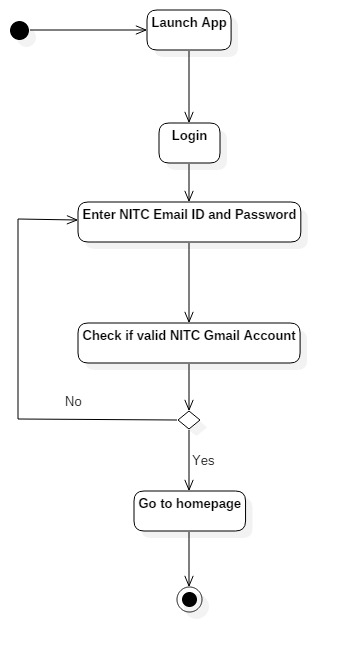
\includegraphics[width=1\textwidth]{activity1}
  \caption{Activity diagram for login activity}
\end{figure}
\begin{figure}[h!]
  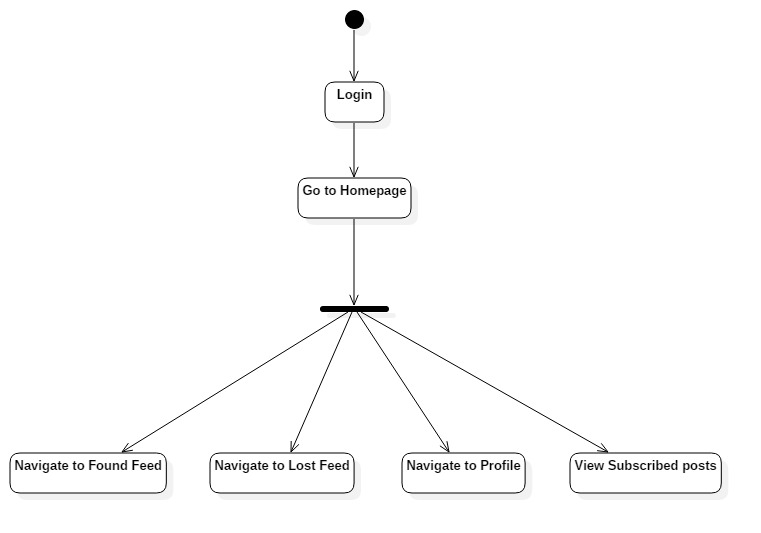
\includegraphics[width=1\textwidth]{activity2}
  \caption{Activity diagram for Homepage}
\end{figure}
\begin{figure}[h!]
  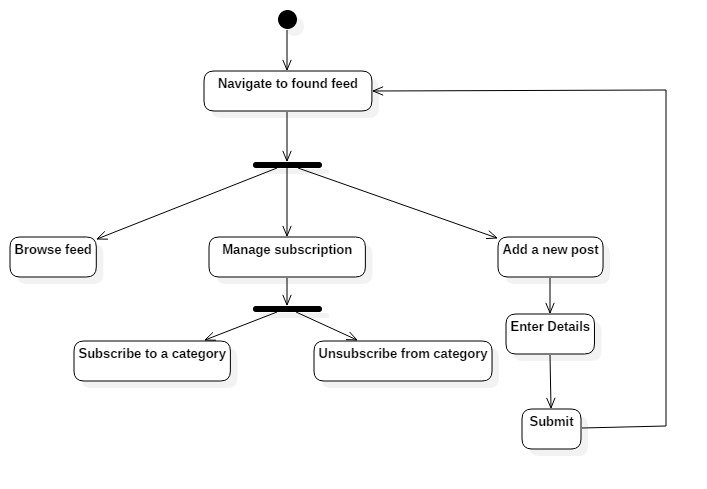
\includegraphics[width=1\textwidth]{activity3}
  \caption{Activity diagram for Navigation to Found feed}
\end{figure}
\begin{figure}[h!]
  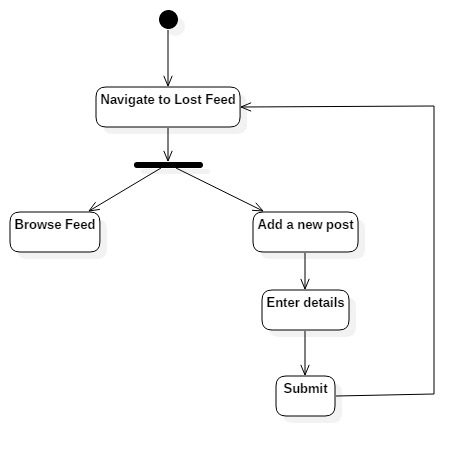
\includegraphics[width=1\textwidth]{activity4}
  \caption{Activity Diagram for Navigation to lost feed}
\end{figure}
\begin{figure}[h!]
  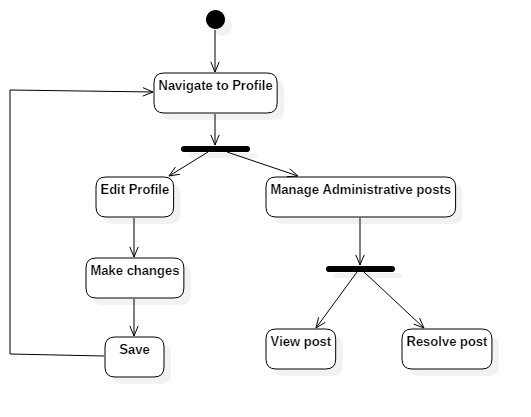
\includegraphics[width=1\textwidth]{activity5}
  \caption{Activity diagram for Navigation to Profile}
\end{figure}
\begin{figure}[h!]
  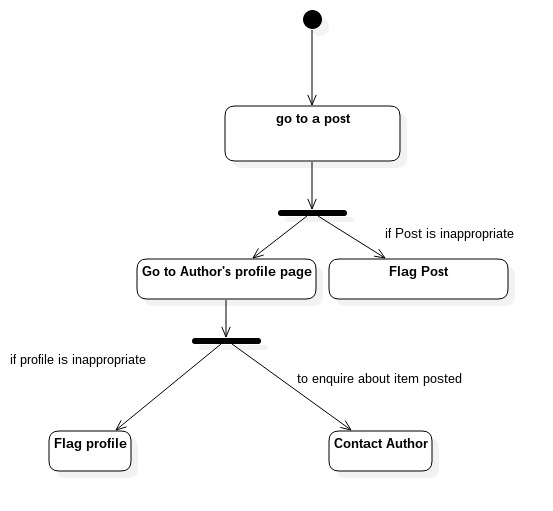
\includegraphics[width=1\textwidth]{activity6}
  \caption{Activity Diagram for Reporting}
\end{figure}
\begin{figure}[h!]
  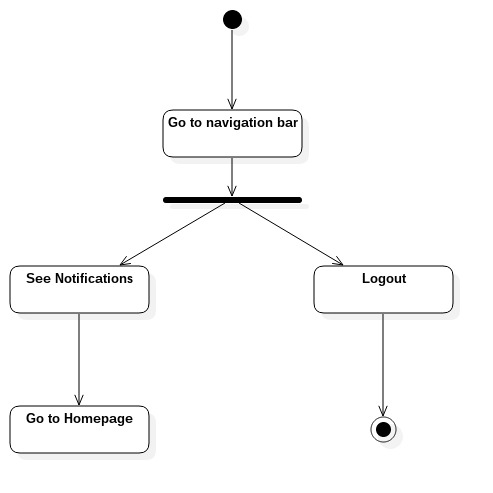
\includegraphics[width=1\textwidth]{activity7}
  \caption{Activity diagram for Logout and Notification}
\end{figure}
}
\subsection{Interface/Exports}
\begin{itemize}
\item Post Details: This component takes the 'item details' and sends it to the database. Exception: if the user abandons this operation before clicking 'Submit', the entry will not be updated in the 'database'. 
\item Resolving a post: This component takes the item id and deletes the entry corresponding to the item in the 'database'.  
\item Reporting a user/item: This component takes the item id/user id and flags the entry corresponding to the item/user in the 'database'. Exception: if the user abandons this operation before confirming, no change is reflected in the system. 
\item Subscribing/unsubscribing a category: This component takes the category id and the user id and updates it in the 'database' so that items feed can be updated accordingly. 
\item Authentication: It takes a Gmail ID and checks if it is present in the database. If founds, it starts a session which allows a user to access all the functionalities. 
\item Database: This component updates/adds information to the 'database' corresponding to that particular user id or item id.
\end{itemize}
\subsection{Detailed Subsystem Design}
As mentioned, the 3 Subsystems in this application are the Application Interface, the Database and the Actions available to the user. All Actions can be processed only with a working Internet Connection, i.e., no data/information is stored locally on the device (other than the session cookies).
\section{Data Design}
\subsection{Database Description}
\begin{figure}[h!]
  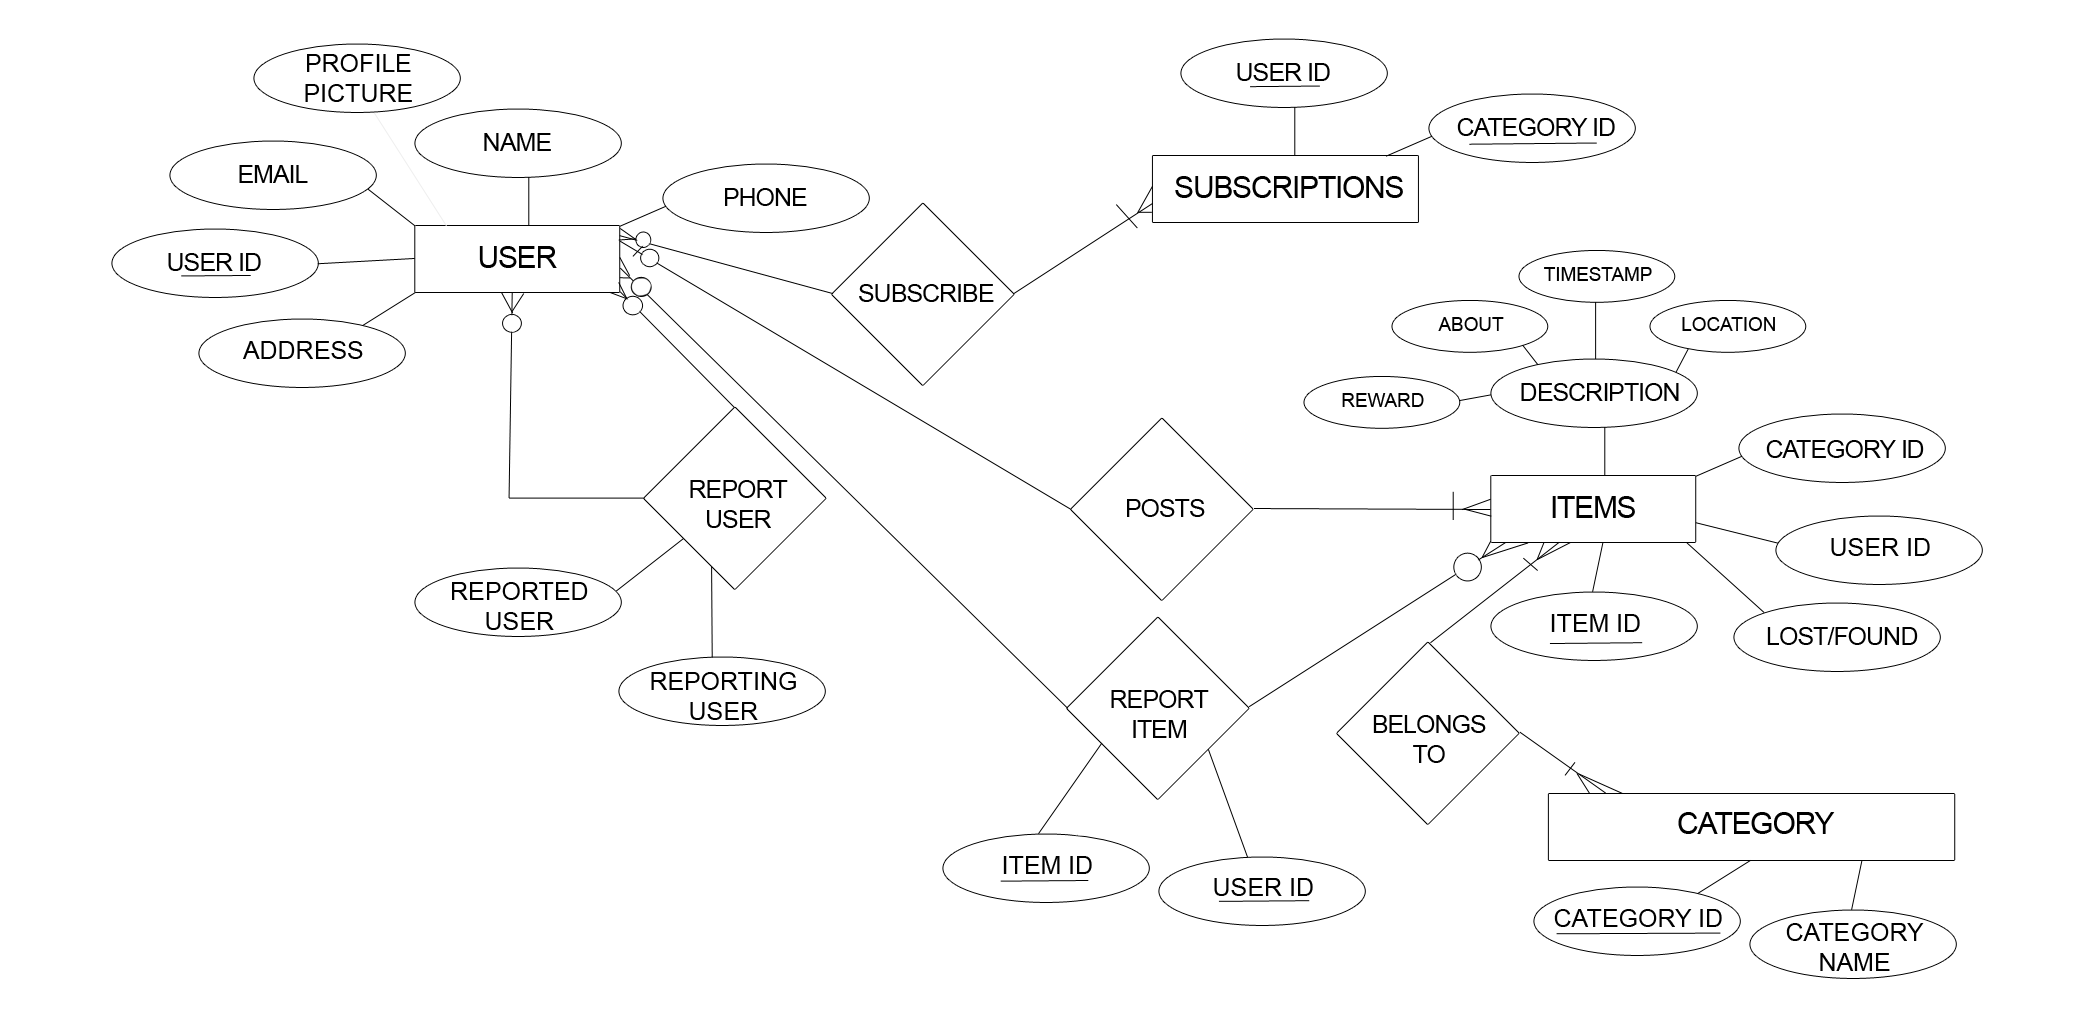
\includegraphics[width=1\textwidth]{erd}
  \caption{ER Diagram for LFA}
\end{figure}
The Entity Relation diagram given in \textbf{Figure 16} has the following entities:\\
 1) User\\
 2) Subscriptions\\
 3) Items\\
 4) Category\\
The attributes of each entities and relationships among entities are shown in the diagram.
\subsection{Global Data Structures}
There are no specific data structures to be used in particular. Arrays could be used for storing the items while matching the Lost and Found products.
\section{Glossary}
\begin{itemize}
\item Database: A structured set of data held in a computer, especially one that is accessible in various ways. 
\item User: A person who uses or operates something (in this case, the user is using the application) 
\item Report: Make a formal statement or complaint about (someone or something) to the necessary authority. 
\item Item: An object of value that has been found by a user, or one that has been lost by someone. 
\item Post: Contains details about an item like the appearance, the location it was found/lost (last seen) and the time-frame when it was found/lost 
\item Subscribe: To ensure that you are notified about all posts pertaining to an item category of interest, you use this option to receive the relevant feed. 
\end{itemize}
\section{Details of Review Session}
\begin{itemize}
\item Comments: Figures were not numbered.\\
Action taken: All the figures were numbered and an appendix given at the end of the page.
\item Comments: General constraints were incorrect.\\
Decision: Some of the constraints were supposed to be in assumptions and dependency section and some were trivial.\\
Action taken: They were correctly placed under assumptions and dependencies or were deleted.
\item Comments: Development method should have described an SDLC model which is more appropriate for the project.\\
Decision: It was discussed with the mentor and decided to explain an SDLC model under this section, preferably waterfall model.\\
Action taken: Waterfall model has been used for the description.
\item Comments: Class diagram is wrong.\\
Action taken: Modified class diagram has been given in Page
\item Comments: Sequence diagrams have to be modified.\\
Action taken: Modified sequence diagram has been given in Page
\item Comments: Activity diagram is wrong.\\
Action taken: New activity diagram has been given in Page
\item Comments: Use case diagram is wrong.\\
Action taken: New use case diagram has been given in Page
\item Comments: ER diagram is wrong\\
Action taken: New ER diagram has been given in Page
\item Comments: State diagram and component diagram is not required.\\
Action taken: They have been removed from the document.
\end{itemize}
\begin{thebibliography}{}
\bibitem{brad}
Brad Appleton. \textit{A Software Design Specification Template}, (brad@bradapp.net)   http://www.bradapp.net.
\bibitem{srs}
Buxbuddy SRS  \textit{version 1.1}
\bibitem{design}
Design Doc Template  \textit{www.se.rit.edu/~vdkrit/design/VDK-RIT\_SDS.doc}
\bibitem{uml}
UML Reference  \textit{http://www.uml-diagrams.org/uml-25-diagrams.html }
\end{thebibliography}{}
\end{document}